\documentclass[tikz,border=10pt]{standalone}
\begin{document}
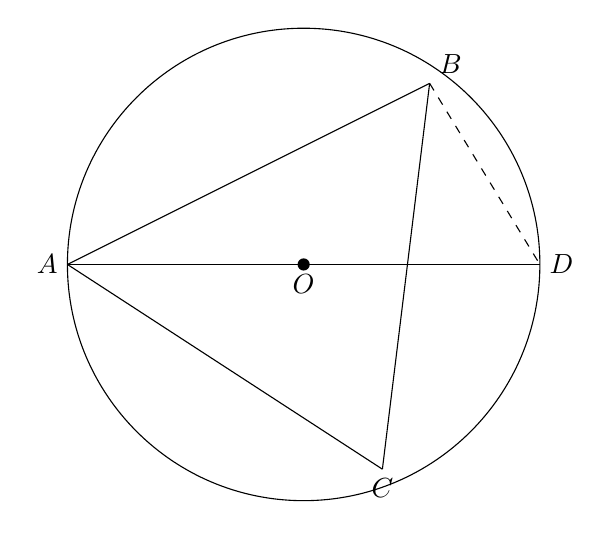
\begin{tikzpicture}[scale=1]

\coordinate (O) at (0,0);
\coordinate (A) at (-3,0);
\coordinate (D) at (3,0);
\coordinate (B) at (1.6,2.3);
\coordinate (C) at (1.0,-2.6);

\draw (O) circle[radius=3];
\draw (A) -- (B);
\draw (A) -- (C);
\draw (A) -- (D);
\draw (B) -- (C);
\draw[dashed] (B) -- (D);

\fill (O) circle[radius=2.2pt];

\node[left] at (A) {$A$};
\node[above right] at (B) {$B$};
\node[below] at (C) {$C$};
\node[right] at (D) {$D$};
\node[below] at (O) {$O$};

\end{tikzpicture}
\end{document}
